% GENERATED by build_chapters.py; edit docs/report/chapters, not this file

\chapter{The ci-heal-backend Service}

\section{Purpose and difference from the n8n healer}

\texttt{ci-\allowbreak{}heal-\allowbreak{}backend} is a FastAPI service that acts as the second healer in this project. It watches for failed GitHub Actions runs, asks a language model what kind of failure it was, and then does one of three things: ask GitHub to re-run the failed jobs, open a pull request with a small fix, or open an issue for a person to read. It starts in a safe mode. \texttt{DRY\_\allowbreak{}RUN} is true by default, so nothing is written to GitHub until the operator sets \texttt{DRY\_\allowbreak{}RUN=false} (source: app/\allowbreak{}config.py).

The first healer is the n8n workflow described in an earlier chapter. It is a chain of workflow nodes that prompts the model and acts on the answer. The backend does the same job as ordinary code with a database behind it. Three differences matter in practice.

\begin{itemize}[leftmargin=*, itemsep=2pt]
\item The decision is made by a pure function, \texttt{decide} in \texttt{app/\allowbreak{}core/\allowbreak{}decision\_\allowbreak{}engine.\allowbreak{}py}, with named thresholds. The model only supplies a category and a confidence. It never chooses the action.
\item Every failure, classification, fix candidate and decision is stored in a database, so attempt budgets, outcomes and calibration statistics can be read back later.
\item A fix is generated several times and the candidates are compared with each other. The pull request is only opened when they agree closely enough.
\end{itemize}

The log trimming rules are a direct port of the \texttt{trimCiLog} function from the n8n "Build AI Prompt" node, so both healers show the model the same kind of log excerpt (source: app/\allowbreak{}core/\allowbreak{}log\_\allowbreak{}trim.py). The two model roles, classifier and fixer, each have their own URL, key and model name, and both can point at the self-hosted Qwen3.8-27B endpoint (source: app/\allowbreak{}config.py).

\section{Request flow}

\begin{figure}[!htbp]
\centering
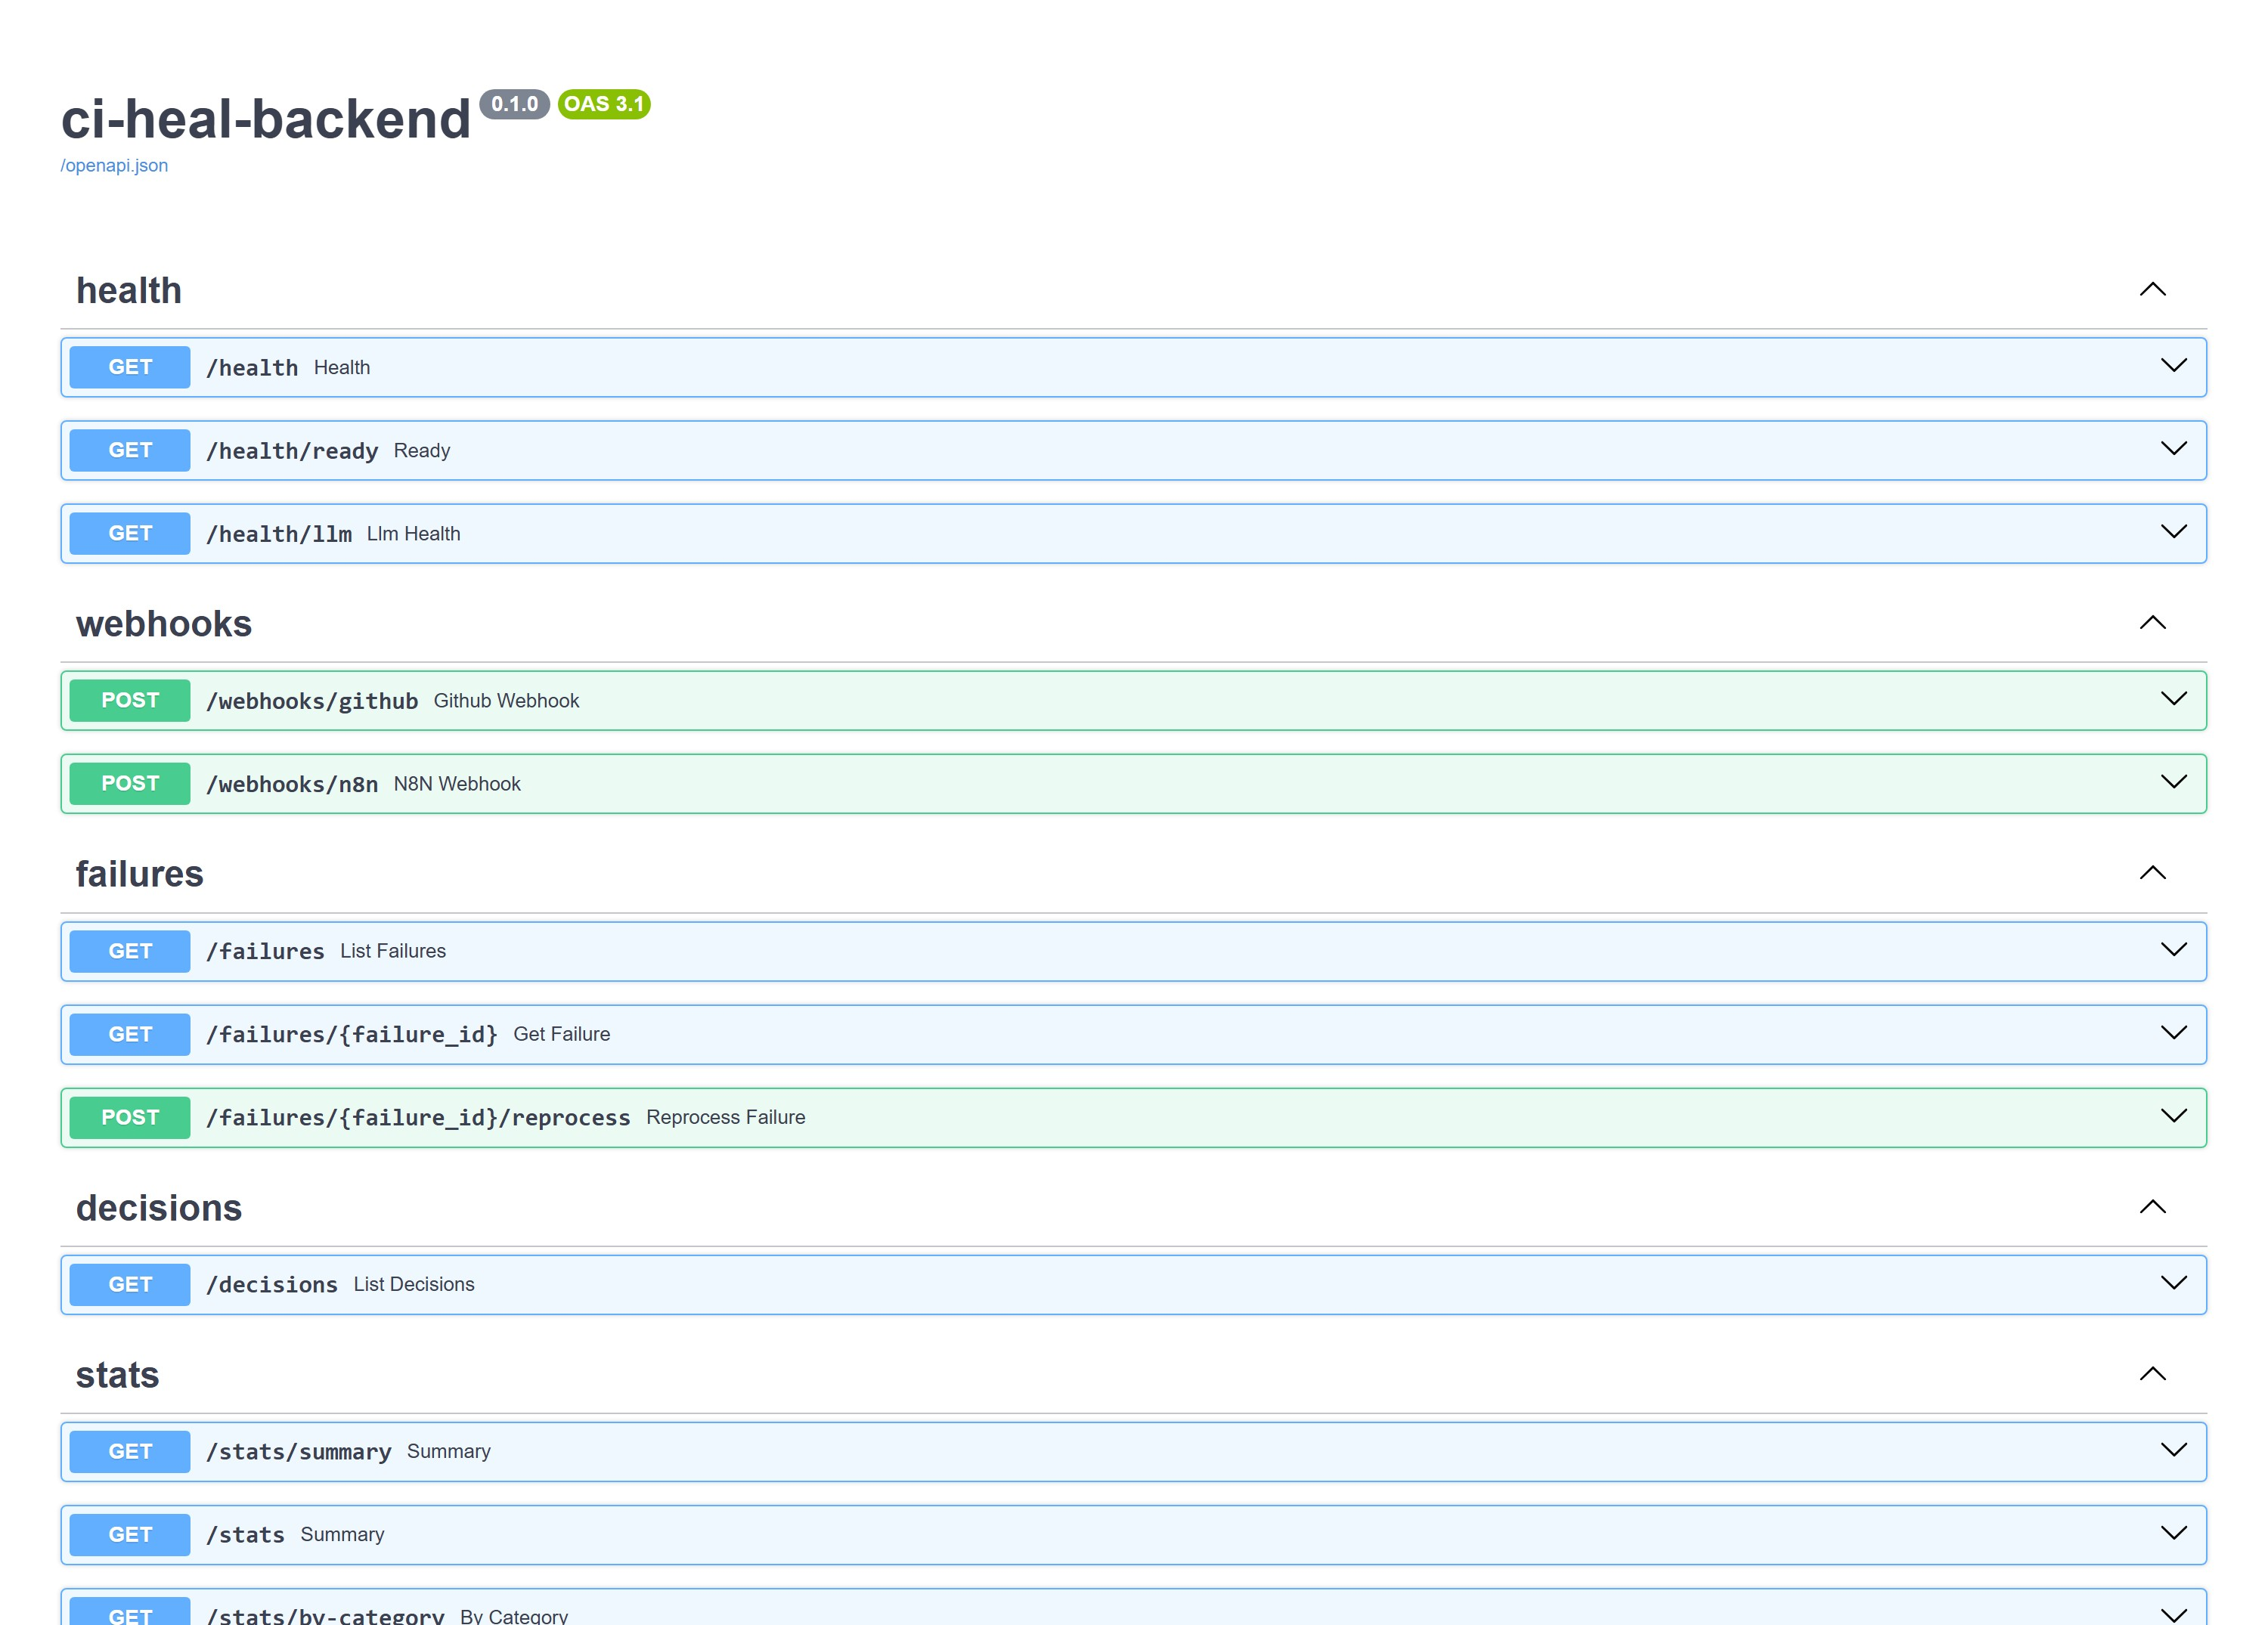
\includegraphics[width=0.88\linewidth]{figures/shots/hq_swagger.jpg}
\caption{The interactive API page of \texttt{ci-heal-backend} (\texttt{/docs}): the health, webhook, failure, decision and statistics endpoints.}
\label{fig:shot-swagger}
\end{figure}


A failure travels through the service in the order below. The numbers refer to the code in \texttt{app/\allowbreak{}api/\allowbreak{}webhooks.\allowbreak{}py} and \texttt{app/\allowbreak{}services/\allowbreak{}orchestrator.\allowbreak{}py}.

\begin{enumerate}[leftmargin=*, itemsep=2pt]
\item \textbf{Webhook.} GitHub posts a \texttt{workflow\_\allowbreak{}run} event to \texttt{POST /\allowbreak{}webhooks/\allowbreak{}github}. n8n can instead post a small JSON body (run id, repo, branch, commit) to \texttt{POST /\allowbreak{}webhooks/\allowbreak{}n8n}, and the backend then loads the real run from the GitHub API. Both routes reduce the delivery to one internal \texttt{IncomingRun} object.
\item \textbf{Authentication.} The GitHub route checks the \texttt{X-\allowbreak{}Hub-\allowbreak{}Signature-\allowbreak{}256} HMAC over the raw body. The n8n route compares the \texttt{X-\allowbreak{}N8N-\allowbreak{}Token} header with \texttt{N8N\_\allowbreak{}SHARED\_\allowbreak{}TOKEN}. A wrong value is a 401. A \texttt{ping} event returns 200.
\item \textbf{Intake rules.} Only a completed run with conclusion \texttt{failure} or \texttt{success} is acted on, and everything else gets 202 with status \texttt{ignored}. The repository must be in \texttt{ALLOWED\_\allowbreak{}REPOS}, and an empty list allows nothing, otherwise the answer is 403. A run on a branch that starts with \texttt{ai-\allowbreak{}fix-\allowbreak{}} is never treated as new work. It is only used to verify an earlier fix. A run whose actor is the token owner (\texttt{GITHUB\_\allowbreak{}BOT\_\allowbreak{}LOGIN}) is ignored, so the bot cannot trigger itself. The body is limited to \texttt{WEBHOOK\_\allowbreak{}MAX\_\allowbreak{}BYTES}, 1,000,000 by default (source: app/\allowbreak{}api/\allowbreak{}webhooks.py, app/\allowbreak{}config.py).
\item \textbf{Claim.} The failure row is unique on repo, run id and run attempt, so a repeated delivery returns \texttt{duplicate}. The row is saved as \texttt{queued}, the request returns 202, and a background task takes over. The worker moves the row to \texttt{processing} with one UPDATE that only matches a row still in \texttt{queued}, so two workers cannot take the same failure (source: app/\allowbreak{}db/\allowbreak{}repositories.py).
\item \textbf{Fetch evidence.} The worker downloads the run log zip, compares the commit with its parent to get a diff, and loads up to eight files that the diff touches. The log token is not forwarded to the redirect host that serves the zip (source: app/\allowbreak{}services/\allowbreak{}github\_\allowbreak{}client.py, app/\allowbreak{}services/\allowbreak{}orchestrator.py).
\item \textbf{Redact and trim.} Secrets in the log, diff and files are replaced with \texttt{[REDACTED:\allowbreak{}\textless{}KIND\textgreater{}]} placeholders first. Only then is the log cut to the failure region: from the last \texttt{\#\#[endgroup]} before the first \texttt{\#\#[error]} line, at most 40 lines and 3000 characters. Redacting first matters because a secret outside the kept region would otherwise escape the count (source: app/\allowbreak{}services/\allowbreak{}secret\_\allowbreak{}redactor.py, app/\allowbreak{}core/\allowbreak{}log\_\allowbreak{}trim.py).
\item \textbf{Classify.} The classifier role returns one of four categories with a confidence. The result is stored as a classification row.
\item \textbf{Decision stage 1.} The engine sees the category, the confidence, the retry count and the attempt count. It answers retry, escalate, or candidate fix.
\item \textbf{Fixer.} For a candidate fix, the fixer role is asked for \texttt{FIX\_\allowbreak{}CANDIDATES} patches (3 by default), one after another, at temperature 0.7. Each reply must be a JSON object with a file path and SEARCH/\allowbreak{}REPLACE edits. Each patch is applied to the original file text in memory and checked by the guards described below. A call that fails or a patch that does not apply becomes an invalid candidate and does not stop the others (source: app/\allowbreak{}services/\allowbreak{}fix\_\allowbreak{}generator.py).
\item \textbf{Agreement and stage 2.} Candidates are scored against each other. The engine runs again with the agreement score and answers fix or escalate.
\item \textbf{Act.} A fix opens a pull request. An escalation opens an issue. A retry asks GitHub to re-run the failed jobs. In dry-run each of these is only logged and a placeholder URL is stored.
\item \textbf{Verify later.} When a later \texttt{workflow\_\allowbreak{}run} arrives, the backend closes the open decision. A re-run of a retried run closes the retry as \texttt{retry\_\allowbreak{}success} or \texttt{retry\_\allowbreak{}failure}. A run on the \texttt{ai-\allowbreak{}fix-\allowbreak{}*} branch closes the fix as \texttt{verified\_\allowbreak{}success} or \texttt{verified\_\allowbreak{}failure}. The whole pipeline for one failure is cut off after \texttt{PIPELINE\_\allowbreak{}TIMEOUT\_\allowbreak{}SECONDS}, 180 by default. If it fails, the row is marked \texttt{error} and the service tries to open an escalation issue (source: app/\allowbreak{}services/\allowbreak{}orchestrator.py).
\end{enumerate}

The agreement score is the mean pairwise similarity of the candidate diffs. For each pair the score is the average of a token Jaccard value and the \texttt{difflib} ratio on the diff with headers removed. An invalid candidate has similarity 0 with every other one and still counts in the mean, so a bad sample pulls the score down. Two valid candidates that edit different files also score 0. If fewer than two candidates applied, there is no score and the decision is escalate. The patch that is published is the medoid, meaning the candidate with the highest mean similarity to the others (source: app/\allowbreak{}core/\allowbreak{}agreement.py).

\section{Failure categories}

The classifier must answer with exactly one of four labels. A fifth label, \texttt{unknown}, exists only for the case where the reply could not be parsed or the samples tied. It always escalates (source: app/\allowbreak{}core/\allowbreak{}enums.py, app/\allowbreak{}core/\allowbreak{}decision\_\allowbreak{}engine.py).

\begingroup\small
\begin{longtable}{>{\raggedright\arraybackslash}p{0.506\dimexpr\linewidth-4\tabcolsep\relax}>{\raggedright\arraybackslash}p{0.494\dimexpr\linewidth-4\tabcolsep\relax}}
\toprule
\rowcolor{gray!14}\textbf{Category} & \textbf{Action when confident} \\
\midrule
\endhead
\bottomrule
\endfoot
\endlastfoot
\texttt{dependency\_\allowbreak{}error} & generate patches, then fix or escalate \\
\texttt{configuration\_\allowbreak{}error} & generate patches, then fix or escalate \\
\texttt{test\_\allowbreak{}failure} & generate patches, then fix or escalate \\
\texttt{flaky\_\allowbreak{}or\_\allowbreak{}network} & re-run the failed jobs, no code change \\
\bottomrule
\caption{Failure categories}\label{tab:08-1}\\
\end{longtable}
\endgroup

\section{Thresholds and attempt budgets}

The defaults below are read from \texttt{app/\allowbreak{}config.\allowbreak{}py}. Each one can be changed with an environment variable of the same name in capitals.

\begingroup\small
\begin{longtable}{>{\raggedright\arraybackslash}p{0.429\dimexpr\linewidth-6\tabcolsep\relax}>{\raggedright\arraybackslash}p{0.143\dimexpr\linewidth-6\tabcolsep\relax}>{\raggedright\arraybackslash}p{0.429\dimexpr\linewidth-6\tabcolsep\relax}}
\toprule
\rowcolor{gray!14}\textbf{Setting} & \textbf{Default} & \textbf{What it controls} \\
\midrule
\endhead
\bottomrule
\endfoot
\endlastfoot
\texttt{CLASSIFY\_\allowbreak{}THRESHOLD} & 0.75 & minimum confidence to go on to a fix \\
\texttt{AGREEMENT\_\allowbreak{}THRESHOLD} & 0.6 & minimum agreement to open a pull request \\
\texttt{FLAKY\_\allowbreak{}THRESHOLD} & 0.75 & minimum confidence to re-run a flaky failure \\
\texttt{MAX\_\allowbreak{}RETRIES} & 1 & re-runs allowed for one run id \\
\texttt{MAX\_\allowbreak{}HEAL\_\allowbreak{}ATTEMPTS} & 3 & fix decisions allowed on one branch before escalating \\
\texttt{CATEGORY\_\allowbreak{}THRESHOLDS} & \texttt{\{\}} & per-category confidence gates that replace the first and third rows \\
\texttt{CLASSIFIER\_\allowbreak{}SAMPLES} & 1 & classifier votes \\
\texttt{FIX\_\allowbreak{}CANDIDATES} & 3 & patches requested \\
\texttt{MAX\_\allowbreak{}RECOVERIES} & 3 & startup requeues per failure \\
\texttt{PROCESSING\_\allowbreak{}STALE\_\allowbreak{}SECONDS} & 900 & age after which a \texttt{processing} row counts as abandoned at startup \\
\bottomrule
\caption{Thresholds and attempt budgets}\label{tab:08-2}\\
\end{longtable}
\endgroup

All comparisons are inclusive. The comment in the config explains why 0.75 was picked: with three classifier samples a two-to-one vote gives about 0.667, which falls under the gate and escalates. With one sample, the model's own confidence is used. With several samples, the stored confidence is the smaller of the mean self-reported confidence and the share of samples that voted for the winning category (source: app/\allowbreak{}config.py, app/\allowbreak{}services/\allowbreak{}classifier.py).

The decision engine checks its rules in a fixed order. Invalid input and \texttt{unknown} escalate first. Then, if the attempt count has reached \texttt{MAX\_\allowbreak{}HEAL\_\allowbreak{}ATTEMPTS}, it escalates. Then the flaky rule applies, and then the fixable rule. The two counters come from the database. \texttt{retries\_\allowbreak{}done} is the number of RETRY decisions stored for the same repository and run id. \texttt{attempt} is the number of FIX decisions on the same repository and failing branch since the last \texttt{verified\_\allowbreak{}success} on that branch (source: app/\allowbreak{}db/\allowbreak{}repositories.py).

\section{Safety rules}

\begin{itemize}[leftmargin=*, itemsep=2pt]
\item \textbf{Branch names.} The backend never uses the name the model proposes. It builds \texttt{ai-\allowbreak{}fix-\allowbreak{}\textless{}category\textgreater{}-\allowbreak{}\textless{}sha7\textgreater{}} itself and creates it from the failing commit. The GitHub client refuses any ref write whose branch does not start with \texttt{ai-\allowbreak{}fix-\allowbreak{}}, or is \texttt{main}, \texttt{master} or the configured default branch, or contains a slash, \texttt{.\allowbreak{}.\allowbreak{}} or whitespace. The refusal is an exception, not an assert, so it survives \texttt{python -\allowbreak{}O}. A failure that is already on an \texttt{ai-\allowbreak{}fix-\allowbreak{}*} branch is refused with \texttt{fix\_\allowbreak{}loop}.
\item \textbf{Protected paths.} A patch may only touch a file that was in the context shown to the model. Absolute paths, \texttt{.\allowbreak{}.\allowbreak{}}, \texttt{.\allowbreak{}git/\allowbreak{}}, \texttt{.\allowbreak{}env*} and \texttt{.\allowbreak{}github/\allowbreak{}workflows/\allowbreak{}} are rejected. The workflow ban can be lifted with \texttt{FIX\_\allowbreak{}ALLOW\_\allowbreak{}WORKFLOWS}, the others cannot.
\item \textbf{Size limits.} At most \texttt{FIX\_\allowbreak{}MAX\_\allowbreak{}EDITS} blocks (5) and \texttt{FIX\_\allowbreak{}MAX\_\allowbreak{}CHANGED\_\allowbreak{}LINES} changed lines (50). Each SEARCH text must match the file exactly once.
\item \textbf{Syntax check.} For a \texttt{.\allowbreak{}py} file the patched text must parse with \texttt{ast.\allowbreak{}parse}. The code is not run.
\item \textbf{Weakened tests.} A patch is rejected if it adds a skip or xfail marker, removes a test function, or removes more assert lines than it adds. Changing an assert in place is allowed.
\item \textbf{Redaction.} Text is redacted before it is stored, before it is sent to a model, and again before the pull request or issue text goes to GitHub. A replacement that contains a secret is rejected. The prompt builder refuses content that is not of the \texttt{RedactedText} type.
\item \textbf{Prompt injection.} Logs, diffs and files are placed between \texttt{\textless{}\textless{}\textless{}UNTRUSTED\_\allowbreak{}.\allowbreak{}.\allowbreak{}.\allowbreak{}\textgreater{}\textgreater{}\textgreater{}} markers, and the system prompt tells the model to treat them as evidence only. The reply schema rejects extra keys (source: app/\allowbreak{}llm/\allowbreak{}prompts.py, app/\allowbreak{}schemas/\allowbreak{}fix.py).
\item \textbf{DRY\_\allowbreak{}RUN.} Every write method of the GitHub client returns before touching the network when dry-run is on. Reads still run. A dry-run decision is flagged in the database and never receives a real CI outcome (source: app/\allowbreak{}services/\allowbreak{}github\_\allowbreak{}client.py, .env.example).
\end{itemize}

(source for this list: app/\allowbreak{}core/\allowbreak{}patch\_\allowbreak{}apply.py, app/\allowbreak{}services/\allowbreak{}github\_\allowbreak{}client.py, app/\allowbreak{}services/\allowbreak{}secret\_\allowbreak{}redactor.py)

\section{The LLM contract and the HTTP client}

\texttt{ci-\allowbreak{}heal-\allowbreak{}backend/\allowbreak{}docs/\allowbreak{}LLM\_\allowbreak{}CONTRACT.\allowbreak{}md} describes what any server must offer. The client in \texttt{app/\allowbreak{}llm/\allowbreak{}http\_\allowbreak{}client.\allowbreak{}py} posts to \texttt{\{root\}/\allowbreak{}v1/\allowbreak{}chat/\allowbreak{}completions} with a bearer token. A base URL that already ends in \texttt{/\allowbreak{}v1} is accepted. Readiness is \texttt{GET /\allowbreak{}v1/\allowbreak{}models}, and any status below 400 counts as up.

The classifier must reply with one JSON object holding \texttt{category}, \texttt{confidence} (0 to 1) and \texttt{reasoning}, with no other keys. The fixer must reply with \texttt{branch\_\allowbreak{}name}, \texttt{file\_\allowbreak{}path}, \texttt{edits}, \texttt{pr\_\allowbreak{}title} and \texttt{pr\_\allowbreak{}body}. A reply may be wrapped in a code fence or a think block, and the client strips both. If the classifier reply does not fit the schema it is asked again, up to \texttt{CLASSIFIER\_\allowbreak{}MAX\_\allowbreak{}RETRIES} (2). After that the verdict is \texttt{unknown} with confidence 0.

Streaming is on by default. The Cloudflare tunnel in front of Kaggle closes a request that stays quiet for about two minutes, so a long completion has to stream. Calls on one client are serialised with a lock, because the Kaggle server runs with \texttt{-\allowbreak{}-\allowbreak{}parallel 1}. Only HTTP 5xx (including 524) and timeouts are retried, within a total deadline per call: \texttt{CLASSIFIER\_\allowbreak{}LLM\_\allowbreak{}DEADLINE} 180 s and \texttt{FIXER\_\allowbreak{}LLM\_\allowbreak{}DEADLINE} 360 s, with per-attempt timeouts of 60 s and 120 s. A 4xx answer is final.

The contract says the client may send \texttt{chat\_\allowbreak{}template\_\allowbreak{}kwargs:\allowbreak{} \{"enable\_\allowbreak{}thinking":\allowbreak{} true\}} on a classifier re-ask. The client does send that field when asked, but reading \texttt{\_\allowbreak{}one\_\allowbreak{}sample} in \texttt{app/\allowbreak{}services/\allowbreak{}classifier.\allowbreak{}py} shows that nothing passes the flag today, so no call turns thinking on. The teammate notes in \texttt{docs/\allowbreak{}backend/\allowbreak{}06-\allowbreak{}status-\allowbreak{}and-\allowbreak{}running.\allowbreak{}md} say the same.

\section{Database tables}

The backend uses SQLAlchemy and creates four tables at startup. SQLite is the default (\texttt{sqlite:\allowbreak{}/\allowbreak{}/\allowbreak{}/\allowbreak{}.\allowbreak{}/\allowbreak{}ci\_\allowbreak{}heal.\allowbreak{}db}) with foreign keys, WAL mode and a 5 second busy timeout. A hosted PostgreSQL URL also works (source: app/\allowbreak{}db/\allowbreak{}models.py, app/\allowbreak{}db/\allowbreak{}session.py).

\begingroup\small
\begin{longtable}{>{\raggedright\arraybackslash}p{0.392\dimexpr\linewidth-4\tabcolsep\relax}>{\raggedright\arraybackslash}p{0.608\dimexpr\linewidth-4\tabcolsep\relax}}
\toprule
\rowcolor{gray!14}\textbf{Table} & \textbf{Holds} \\
\midrule
\endhead
\bottomrule
\endfoot
\endlastfoot
\texttt{failures} & one row per run attempt: repo, run id, attempt, branch, commit, actor, status (\texttt{queued}, \texttt{processing}, \texttt{done}, \texttt{error}), redacted log excerpt, redaction count, recovery count \\
\texttt{classifications} & category, confidence, reasoning, model name, raw output, every sample, parse attempts, latency \\
\texttt{fix\_\allowbreak{}candidates} & candidate index, file path, edits, whether it applied, error code, diff \\
\texttt{decisions} & action, category, confidence, agreement, reason code, a snapshot of the thresholds, \texttt{dry\_\allowbreak{}run}, expected run attempt, fix branch, PR and issue URLs, outcome \\
\bottomrule
\caption{Database tables}\label{tab:08-3}\\
\end{longtable}
\endgroup

The thresholds snapshot is stored with each decision, so a later change of configuration does not rewrite the reasons for an old decision. The read API (\texttt{/\allowbreak{}failures}, \texttt{/\allowbreak{}decisions}, \texttt{/\allowbreak{}stats/\allowbreak{}.\allowbreak{}.\allowbreak{}.\allowbreak{}}) needs \texttt{API\_\allowbreak{}TOKEN} outside dev.

\section{Wiring to the Kaggle endpoint}

\texttt{kaggle/\allowbreak{}tools/\allowbreak{}backend\_\allowbreak{}env.\allowbreak{}py} points both roles at the live endpoint. It reads the tunnel URL from the file \texttt{\%LOCALAPPDATA\%\textbackslash{}selfheal-\allowbreak{}n8n\textbackslash{}qwen\_\allowbreak{}url.\allowbreak{}txt} and the key from \texttt{kaggle/\allowbreak{}endpoint/\allowbreak{}deploy\_\allowbreak{}src.\allowbreak{}py}, then rewrites only the \texttt{PROVIDER}, \texttt{BASE\_\allowbreak{}URL}, \texttt{API\_\allowbreak{}KEY} and \texttt{MODEL} lines of both roles in \texttt{ci-\allowbreak{}heal-\allowbreak{}backend/\allowbreak{}.\allowbreak{}env}. Every other line is kept. With \texttt{-\allowbreak{}-\allowbreak{}check} it also calls \texttt{GET /\allowbreak{}v1/\allowbreak{}models}. The key is never printed, and \texttt{.\allowbreak{}env} is ignored by git.

Qwen3.8's chat template thinks unless told not to. The backend only ever sends \texttt{enable\_\allowbreak{}thinking} to switch thinking on, so before the change every call would have thought first, and thinking tokens count against the 512 token classifier limit. The endpoint now starts llama-server with thinking off by default, and a boot check asks the same question twice to confirm that the default is off and that \texttt{enable\_\allowbreak{}thinking:\allowbreak{} true} still turns it on (source: docs/\allowbreak{}results/\allowbreak{}BACKEND\_\allowbreak{}ON\_\allowbreak{}KAGGLE.md).

\section{Measured replay on the endpoint}

On 2026-11-15 the six fixtures in \texttt{ci-\allowbreak{}heal-\allowbreak{}backend/\allowbreak{}fixtures/\allowbreak{}} were replayed through the real pipeline with \texttt{scripts/\allowbreak{}replay\_\allowbreak{}failure.\allowbreak{}py -\allowbreak{}-\allowbreak{}llm http}. GitHub was mocked and \texttt{DRY\_\allowbreak{}RUN} was on. The endpoint was the unsloth UD-Q4\_\allowbreak{}K\_\allowbreak{}XL build on two T4 GPUs at 26.8 tokens per second (source: docs/\allowbreak{}results/\allowbreak{}BACKEND\_\allowbreak{}ON\_\allowbreak{}KAGGLE.md).

\begingroup\small
\begin{longtable}{>{\raggedright\arraybackslash}p{0.239\dimexpr\linewidth-10\tabcolsep\relax}>{\raggedright\arraybackslash}p{0.312\dimexpr\linewidth-10\tabcolsep\relax}>{\raggedright\arraybackslash}p{0.217\dimexpr\linewidth-10\tabcolsep\relax}>{\raggedright\arraybackslash}p{0.159\dimexpr\linewidth-10\tabcolsep\relax}>{\raggedright\arraybackslash}p{0.072\dimexpr\linewidth-10\tabcolsep\relax}}
\toprule
\rowcolor{gray!14}\textbf{Fixture} & \textbf{Classified (confidence)} & \textbf{Decision} & \textbf{Candidates applied} & \textbf{Time} \\
\midrule
\endhead
\bottomrule
\endfoot
\endlastfoot
configuration & configuration\_\allowbreak{}error (0.95) & fix & 3 of 3 & 28 s \\
dependency & dependency\_\allowbreak{}error (0.98) & escalate, candidates disagreed & 3 of 3 & 30 s \\
flaky & flaky\_\allowbreak{}or\_\allowbreak{}network (0.95) & re-run the job & not asked for & 8 s \\
prompt\_\allowbreak{}injection & test\_\allowbreak{}failure (0.98) & fix, agreement 1.0 & 3 of 3 & 26 s \\
secrets & dependency\_\allowbreak{}error (0.98), 2 secrets redacted & escalate, candidates disagreed & 3 of 3 & 40 s \\
test\_\allowbreak{}failure & test\_\allowbreak{}failure (0.98) & fix & 3 of 3 & 29 s \\
\bottomrule
\caption{Measured replay on the endpoint}\label{tab:08-4}\\
\end{longtable}
\endgroup

All six were classified correctly on the first sample and all 15 candidates that were asked for applied to the file. Two cases escalated because the three dependency patches differed and agreement fell below 0.6. That is the gate doing its job, but the replay cannot say which patch would have fixed the build. The limits are plain: one run per fixture, six fixtures written for the backend's own tests, no pull request opened, and no CI run on a fix. The replay output also does not show whether any candidate followed the injected text in the prompt-injection fixture.

\section{Tests}

The tests run offline with a mock model and a mocked GitHub client. At the last commit, \texttt{python -\allowbreak{}m pytest -\allowbreak{}q} in \texttt{ci-\allowbreak{}heal-\allowbreak{}backend} collected and passed 157 tests in 16 test modules (run on an export of that commit, in about 17 seconds). The modules cover the decision engine, agreement scoring, patch application, secret redaction, log trimming, the classifier and fix generator, the HTTP LLM client, the GitHub client, the repositories and statistics, the webhooks, health endpoints, settings, and a test that \texttt{.\allowbreak{}env.\allowbreak{}example} keeps the same keys as \texttt{Settings}. The working tree contains a new \texttt{tests/\allowbreak{}test\_\allowbreak{}security.\allowbreak{}py} and edits to \texttt{tests/\allowbreak{}test\_\allowbreak{}webhooks.\allowbreak{}py} for the audit fixes below, so a count taken now differs from 157.

\section{Known limitations from an audit}

A read-only security review of the code produced 21 findings. Each one below was checked again against the code for this chapter, and all 21 were confirmed by reading it. None was reproduced by running a failing request. The wording of each row says what the code does, not what was observed live.

\begingroup\small
\begin{longtable}{>{\raggedright\arraybackslash}p{0.069\dimexpr\linewidth-6\tabcolsep\relax}>{\raggedright\arraybackslash}p{0.414\dimexpr\linewidth-6\tabcolsep\relax}>{\raggedright\arraybackslash}p{0.517\dimexpr\linewidth-6\tabcolsep\relax}}
\toprule
\rowcolor{gray!14}\textbf{No.} & \textbf{Finding, as read from the code} & \textbf{Where} \\
\midrule
\endhead
\bottomrule
\endfoot
\endlastfoot
1 & The run's origin is not checked. Neither \texttt{\_\allowbreak{}from\_\allowbreak{}github} nor \texttt{\_\allowbreak{}from\_\allowbreak{}api} reads the head repository or the triggering event, so a workflow run from a fork pull request can reach the bot. & app/\allowbreak{}api/\allowbreak{}webhooks.py \\
2 & The worker flushes a write on the shared SQLite file and then awaits model and GitHub calls before it commits. Webhook intake is an \texttt{async def} that makes synchronous database calls on the event loop. A second delivery can wait on the lock in the loop thread, blocking the worker that holds it, until the 5 second busy timeout gives "database is locked". & app/\allowbreak{}services/\allowbreak{}orchestrator.py, app/\allowbreak{}api/\allowbreak{}webhooks.py, app/\allowbreak{}db/\allowbreak{}session.py \\
3 & A failure can stay in \texttt{processing} after a restart. Startup recovery skips a \texttt{processing} row that started less than 900 seconds earlier, and it runs only at startup. A cancelled worker task is not caught by \texttt{except Exception} in \texttt{Orchestrator.\allowbreak{}run}, so the row is never moved on. & app/\allowbreak{}db/\allowbreak{}repositories.py, app/\allowbreak{}main.py \\
4 & The worker commits once at the end. If the run times out or raises after a pull request was opened on GitHub, \texttt{\_\allowbreak{}fail} rolls back and the decision row holding the PR URL is lost. & app/\allowbreak{}services/\allowbreak{}orchestrator.py \\
5 & A fix is closed by the first finished run found on its branch. \texttt{find\_\allowbreak{}open\_\allowbreak{}fix} matches on repo and branch only, and neither the commit nor the workflow is compared. & app/\allowbreak{}api/\allowbreak{}webhooks.py, app/\allowbreak{}db/\allowbreak{}repositories.py \\
6 & Attempt budgets count rows, not outcomes. \texttt{count\_\allowbreak{}fix\_\allowbreak{}attempts} and \texttt{count\_\allowbreak{}retries} count every FIX or RETRY row, including dry-run rows and rows whose GitHub action failed. & app/\allowbreak{}db/\allowbreak{}repositories.py \\
7 & \texttt{find\_\allowbreak{}open\_\allowbreak{}retry} has no \texttt{dry\_\allowbreak{}run} filter, so a dry-run retry row can be closed by a real run. & app/\allowbreak{}db/\allowbreak{}repositories.py \\
8 & Defaults fail open outside Docker. \texttt{APP\_\allowbreak{}ENV} defaults to \texttt{dev}, where an empty webhook secret accepts unsigned deliveries and an empty \texttt{API\_\allowbreak{}TOKEN} leaves the read API open. Nothing rejects placeholder secrets, and a test loads \texttt{.\allowbreak{}env.\allowbreak{}example} values such as \texttt{replace-\allowbreak{}me} into \texttt{Settings}. The Dockerfile sets \texttt{APP\_\allowbreak{}ENV=prod}, which closes both. & app/\allowbreak{}config.py, app/\allowbreak{}api/\allowbreak{}webhooks.py, app/\allowbreak{}deps.py, tests/\allowbreak{}test\_\allowbreak{}env\_\allowbreak{}example.py \\
9 & A null conclusion is treated as failure on the n8n route. \texttt{\_\allowbreak{}from\_\allowbreak{}api} replaces a non-string conclusion with \texttt{failure}. The GitHub route ignores it. & app/\allowbreak{}api/\allowbreak{}webhooks.py \\
10 & A non-ASCII header makes \texttt{compare\_\allowbreak{}digest} raise. The length check passes for an equal-length value, then \texttt{hmac.\allowbreak{}compare\_\allowbreak{}digest} raises \texttt{TypeError} on a non-ASCII string, giving a 500 instead of a 401. & app/\allowbreak{}security.py \\
11 & The request body is read in full by \texttt{request.\allowbreak{}body()} before the \texttt{WEBHOOK\_\allowbreak{}MAX\_\allowbreak{}BYTES} check. & app/\allowbreak{}api/\allowbreak{}webhooks.py \\
12 & Only \texttt{httpx.\allowbreak{}TimeoutException} is caught, in both the GitHub client and the LLM client. Other transport errors, such as a refused connection, escape the retry loop. & app/\allowbreak{}services/\allowbreak{}github\_\allowbreak{}client.py, app/\allowbreak{}llm/\allowbreak{}http\_\allowbreak{}client.py \\
13 & Rate-limit waits are unbounded. The delay comes from \texttt{Retry-\allowbreak{}After} or \texttt{X-\allowbreak{}RateLimit-\allowbreak{}Reset} with no upper cap. & app/\allowbreak{}services/\allowbreak{}github\_\allowbreak{}client.py \\
14 & Non-idempotent POSTs are retried. The same loop retries 5xx and timeouts for every method, including creating a ref, a pull request, an issue and labels. & app/\allowbreak{}services/\allowbreak{}github\_\allowbreak{}client.py \\
15 & The default timeouts do not add up. The pipeline limit is 180 s, while the classifier deadline alone is 180 s and the fixer deadline is 360 s, before any GitHub reads. & app/\allowbreak{}config.py \\
16 & Zip size caps are applied after decompression. \texttt{\_\allowbreak{}unzip} calls \texttt{archive.\allowbreak{}read} on a whole member before it compares with the cap. & app/\allowbreak{}services/\allowbreak{}github\_\allowbreak{}client.py \\
17 & The issue dedup marker is \texttt{ci-\allowbreak{}heal-\allowbreak{}failure-\allowbreak{}\textless{}id\textgreater{}}, a database row id, searched without an open-only filter. After a database reset, a new failure can match an old issue. & app/\allowbreak{}services/\allowbreak{}github\_\allowbreak{}text.py, app/\allowbreak{}services/\allowbreak{}github\_\allowbreak{}client.py \\
18 & The published file path is the raw model string. Patch checking normalises the path, but the pull request service commits \texttt{chosen.\allowbreak{}file\_\allowbreak{}path} as the model wrote it. & app/\allowbreak{}services/\allowbreak{}orchestrator.py, app/\allowbreak{}services/\allowbreak{}fix\_\allowbreak{}generator.py \\
19 & Non-UTF-8 files are corrupted on commit. \texttt{get\_\allowbreak{}file} decodes with \texttt{errors="replace"}, and the patched text is written back as UTF-8. & app/\allowbreak{}services/\allowbreak{}github\_\allowbreak{}client.py \\
20 & Logs lack tracebacks and delivery ids. Failures are logged as the exception class name only, there is no \texttt{exc\_\allowbreak{}info}, and the \texttt{X-\allowbreak{}GitHub-\allowbreak{}Delivery} header is never read. & app/\allowbreak{}services/\allowbreak{}orchestrator.py, app/\allowbreak{}api/\allowbreak{}webhooks.py \\
21 & \texttt{GET /\allowbreak{}health/\allowbreak{}llm} has no authentication dependency. It only reports \texttt{ok} or \texttt{error} for each role. & app/\allowbreak{}api/\allowbreak{}health.py \\
\bottomrule
\caption{Known limitations from an audit}\label{tab:08-5}\\
\end{longtable}
\endgroup

Items 1, 8, 9 and 10 are being fixed with tests in this same change. A status table in \texttt{docs/\allowbreak{}results/\allowbreak{}BACKEND\_\allowbreak{}AUDIT.\allowbreak{}md} records the outcome. The other 17 items are open.
